\chapter{Specifikacija programske potpore}
		
	\section{Funkcionalni zahtjevi}
			
			%\textbf{\textit{dio 1. revizije}}\\
			
			%\textit{Navesti \textbf{dionike} koji imaju \textbf{interes u ovom sustavu} ili  \textbf{su nositelji odgovornosti}. To su prije svega korisnici, ali i administratori sustava, naručitelji, razvojni tim.}\\
				
			%\textit{Navesti \textbf{aktore} koji izravno \textbf{koriste} ili \textbf{komuniciraju sa sustavom}. Oni mogu imati inicijatorsku ulogu, tj. započinju određene procese u sustavu ili samo sudioničku ulogu, tj. obavljaju određeni posao. Za svakog aktora navesti funkcionalne zahtjeve koji se na njega odnose.}\\
			
			
			\noindent \textbf{Dionici:}
			
			\begin{packed_enum}
				
				\item Korisnici
				\item[]\begin{packed_enum}
					\item Neregistrirani korisnici
					\item Klijenti
					\item Kulinarski entuzijasti
					\item Nutricionisti
				\end{packed_enum}
				\item Administratori
				\item Razvojni tim
				
			\end{packed_enum}
			
			\noindent \textbf{Aktori i njihovi funkcionalni zahtjevi:}
			
			\begin{packed_enum}
				\item  \underbar{Neregistrirani korisnik (inicijator) može:}
				
				\begin{packed_enum}
					
					\item Pregledavati kuharice sortirane po novosti na prednjoj stranici
					\item Poslati zahtjev za registraciju:
					\begin{packed_enum}
						
						\item  Za klijenta s korisničkim imenom, lozinkom te imenom i prezimenom 
						\item  Za kulinarskog entuzijasta ili nutricionista sa dodatnom slikom, e-adresom i kratkom biografijom
				
					\end{packed_enum}
					\item  Pretraživati profile kulinarskih entuzijasta
					\item Pretraživati i anonimno komentirati kuharice
					
				\end{packed_enum}

				\item  \underbar{Klijent (inicijator) može:}
				
				\begin{packed_enum}
					
					\item Sve što i neregistrirani korisnik, osim slanja zahtjeva zahtjeva za registraciju
					\item Odabrati dijetu koju prate
					\item Pretraživati recepte skeniranjem QR koda proizvoda
					\item Označiti konzumirane recepte
					\item Komentirati kuharice
					
				\end{packed_enum}
				
				\item  \underbar{Kulinarski entuzijast (inicijator) može:}
				
				\begin{packed_enum}
					
					\item Sve što i klijent
					\item Kreirati recepte i kuharice, to jest tematski povezane skupove recepata
					
				\end{packed_enum}

				\item  \underbar{Nutricionist (inicijator) može:}
				
				\begin{packed_enum}
					
					\item Sve što i klijent
					\item Unositi informacije o proizvodima
					\item Kategorizirati proizvode
					\item Kreirati dijete
					
				\end{packed_enum}

				\item  \underbar{Administrator (inicijator) može:}
				
				\begin{packed_enum}
					
					\item Sve što i klijent, nutricionist i kulinarski entuzijast
					\item Odobriti prijave nutricionista i kulinarskih entuzijasta
					\item Pisati u i čitati iz baze podataka
					
				\end{packed_enum}

				\item  \underbar{Baza podataka (sudionik) može:}
	
				\begin{packed_enum}
					
					\item Brinuti se da je zadovoljen model podataka
					\item čuvati trenutno stanje korisnika, kuharica, dijeti i recepata
					
				\end{packed_enum}
			\end{packed_enum}
			
			\eject 

%			\begin{packed_enum}
%				\item  \underbar{Aktor 1 (inicijator) može:}
%				
%				\begin{packed_enum}
%					
%					\item funkcionalnost 1
%					\item funkcionalnost 2
%					\begin{packed_enum}
%						
%						\item  podfunkcionalnost 1 
%						\item  podfunkcionalnost 2
%				
%					\end{packed_enum}
%					\item  funkcionalnost 3
%					
%				\end{packed_enum}
%			
%				\item  \underbar{Aktor 2 (sudionik) može:}
%				
%				\begin{packed_enum}
%					
%					\item funkcionalnost 1
%					\item funkcionalnost 2
%					
%				\end{packed_enum}
%			\end{packed_enum}
%			
%			\eject 

				
			\subsection{Obrasci uporabe}
%				
%				\textbf{\textit{dio 1. revizije}}
%				
				\subsubsection{Opis obrazaca uporabe}
					\noindent \underbar{\textbf{UC1 - Pregled novih kuharica}}
					\begin{packed_item}
	
						\item \textbf{Glavni sudionik: }Neregistrirani korisnik, Klijent, Kulinarski entuzijast, Administrator
						\item  \textbf{Cilj:} Pregledavanje kuharica
						\item  \textbf{Sudionici:} Baza podataka
						\item  \textbf{Preduvjet:} -
						\item  \textbf{Opis osnovnog tijeka:} 
						
						\item[] \begin{packed_enum}
	
							\item Nove kuharice su prikazane prilikom učitavanja aplikacije
							\item Korisnik odabire jednu od navedenih kuharica
							\item Prikazuje se lista recepata unutar navedene kuharice
						\end{packed_enum}
						
						\item  \textbf{Opis mogućih odstupanja:}
						
						\item[] \begin{packed_item}
	
							\item[2.a] Nema kuharica u bazi podataka
							\item[] \begin{packed_enum}
								
								\item Sustav ispisuje poruku da nema kuharica u bazi podataka
								
							\end{packed_enum}

							
						\end{packed_item}
					\end{packed_item}



					\noindent \underbar{\textbf{UC2 - Registracija klijenta}}
					\begin{packed_item}
	
						\item \textbf{Glavni sudionik: }Neregistrirani korisnik
						\item  \textbf{Cilj:} Stvaranje korisničkog računa s statusom klijenta
						\item  \textbf{Sudionici:} Baza podataka
						\item  \textbf{Preduvjet:} -
						\item  \textbf{Opis osnovnog tijeka:} 
						
						\item[] \begin{packed_enum}
	
							\item pritiskom na gumb "Sign up" otvara se sučelje za registraciju
							\item Korisnik unosi podatke o korisničkom imenu, lozinki, imenu i prezimenu
							\item Korisnik prima obavijest o uspješnoj registraciji
						\end{packed_enum}
						
						\item  \textbf{Opis mogućih odstupanja:}
						
						\item[] \begin{packed_item}
	
							\item[2.a] Odabir već zauzetog korisničkog imena, unos korisničkog podatka u nedozvoljenom formatu
							\item[] \begin{packed_enum}
								
								\item Sustav obavještava korisnika o neuspjeloj registraciji i vraća ga u sučelje za registraciju
								\item Korisnik mijenja potrebne podatke i završava registraciju ili odustaje od registracije
								
							\end{packed_enum}

							
						\end{packed_item}
					\end{packed_item}



					\noindent \underbar{\textbf{UC3 - Registracija kulinarskog entuzijasta ili nutricionista}}
					\begin{packed_item}
	
						\item \textbf{Glavni sudionik: }Neregistrirani korisnik
						\item  \textbf{Cilj:} Stvaranje korisničkog računa s statusom kulinarskog entuzijasta ili nutricionista
						\item  \textbf{Sudionici:} Baza podataka, Administrator
						\item  \textbf{Preduvjet:} -
						\item  \textbf{Opis osnovnog tijeka:} 
						
						\item[] \begin{packed_enum}
	
							\item pritiskom na gumb "Sign up" otvara se sučelje za registraciju
							\item Korisnik unosi podatke o korisničkom imenu, lozinki, imenu i prezimenu, e-adresom, kratkom biografijom i slikom
							\item Korisnik prima obavijest o uspješnoj registraciji nakon odobrenja administratora
						\end{packed_enum}
						
						\item  \textbf{Opis mogućih odstupanja:}
						
						\item[] \begin{packed_item}
	
							\item[2.a] Odabir već zauzetog korisničkog imena i/ili e-maila, unos korisničkog podatka u nedozvoljenom formatu
							\item[] \begin{packed_enum}
								
								\item Sustav obavještava korisnika o neuspjeloj registraciji i vraća ga u sučelje za registraciju
								\item Korisnik mijenja potrebne podatke i završava registraciju ili odustaje od registracije
								
							\end{packed_enum}
							\item[2.b] Administrator ne odobrava registraciju
							\item[] \begin{packed_enum}
								
								\item Sustav obavještava korisnika o neuspjeloj registraciji i vraća ga u sučelje za registraciju
								\item Korisnik mijenja potrebne podatke i završava registraciju ili odustaje od registracije
								
							\end{packed_enum}
							
						\end{packed_item}
					\end{packed_item}



					\noindent \underbar{\textbf{UC4 - Pregled profila kulinarskih entuzijasta}}
					\begin{packed_item}
	
						\item \textbf{Glavni sudionik: }Neregistrirani korisnik, Klijent, Kulinarski entuzijast, Nutricionist, Administrator
						\item  \textbf{Cilj:} Pregled profila kulinarskih entuzijasta
						\item  \textbf{Sudionici:} Baza podataka
						\item  \textbf{Preduvjet:} -
						\item  \textbf{Opis osnovnog tijeka:} 
						
						\item[] \begin{packed_enum}
	
							\item korisnik odabire ime kulinarskog entuzijasta unutar kuharice
							\item Otvara se sučelje s podatcima o kulinarskom entuzijastu
						\end{packed_enum}
						

					\end{packed_item}



					\noindent \underbar{\textbf{UC5 - Pretraživanje profila kulinarskih entuzijasta i kuharica}}
					\begin{packed_item}
	
						\item \textbf{Glavni sudionik: }Neregistrirani korisnik, Klijent, Kulinarski entuzijast, Nutricionist, Administrator
						\item  \textbf{Cilj:} Pregled profila i kuharica koje sadrže ključnu riječ
						\item  \textbf{Sudionici:} Baza podataka
						\item  \textbf{Preduvjet:} -
						\item  \textbf{Opis osnovnog tijeka:} 
						
						\item[] \begin{packed_enum}
	
							\item korisnik u tražilicu upisuje jednu ili više ključnih riječi 
							\item Korisnik odabire gumb za pretraživanje
							\item Otvara se sučelje s listom profila i kuharica koje sadrže ključne riječi
						\end{packed_enum}
						
						\item  \textbf{Opis mogućih odstupanja:}
						
						\item[] \begin{packed_item}
	
							\item[2.a] Niti jedan profil ili kuharica ne sadrži ključnu riječ
							\item[] \begin{packed_enum}
								
								\item Sustav obavještava korisnika o neuspjelom pretraživanju 
								\item Klijent se vrati u sučelje gdje je bio prije pretraživanja
								
							\end{packed_enum}

							\item[2.b] Nije upisana ključna riječ prije pretraživanja
							\item[] \begin{packed_enum}
								
								\item Sustav obavještava korisnika o neuspjelom pretraživanju 
								\item Klijent se vrati u sučelje gdje je bio prije pretraživanja
								
							\end{packed_enum}							
						\end{packed_item}
					\end{packed_item}



					\noindent \underbar{\textbf{UC6 - Anonimno komentiranje kuharica}}
					\begin{packed_item}
	
						\item \textbf{Glavni sudionik: }Neregistrirani korisnik
						\item  \textbf{Cilj:} Komentiranje kuharica
						\item  \textbf{Sudionici:} Baza podataka
						\item  \textbf{Preduvjet:} -
						\item  \textbf{Opis osnovnog tijeka:} 
						
						\item[] \begin{packed_enum}
	
							\item korisnik unutar kuharice odabire gumb "Komentiraj"
							\item Otvara se sučelje gdje korisnik upisuje tekst
							\item Pritiskom na gumb "Spremi", komentar se sprema u bazu podataka i vidljiv je unutar kuharice
						\end{packed_enum}
						
						\item  \textbf{Opis mogućih odstupanja:}
						
						\item[] \begin{packed_item}
	
							\item[2.a] Pokušaj spremanja praznog komentara
							\item[] \begin{packed_enum}
								
								\item Sustav obavještava korisnika o neuspjelom pokušaju spremanja komentara 
								\item Klijent ispuni polje za komentar ili odustane
								
							\end{packed_enum}

						\end{packed_item}
					\end{packed_item}



					\noindent \underbar{\textbf{UC7 - Prijava u sustav}}
					\begin{packed_item}
	
						\item \textbf{Glavni sudionik: } Klijent, Kulinarski entuzijast, Nutricionist, Administrator
						\item  \textbf{Cilj:} Prijava u sustav kao registrirani korisnik
						\item  \textbf{Sudionici:} Baza podataka
						\item  \textbf{Preduvjet:} Registracija profila
						\item  \textbf{Opis osnovnog tijeka:} 
						
						\item[] \begin{packed_enum}
	
							\item Korisnik odabire opciju "Prijavi se"
							\item Korisnik ispunjava potrebne podatke
							\item Korisnik je prijavljen i vraća se na početnu stranicu
						\end{packed_enum}
						
						\item  \textbf{Opis mogućih odstupanja:}
						
						\item[] \begin{packed_item}
	
							\item[2.a] Neispravni unos podataka
							\item[] \begin{packed_enum}
								
								\item Sustav obavještava korisnika o neispravnim podatcima i traži ponovni unos podataka
								
							\end{packed_enum}

						\end{packed_item}
					\end{packed_item}


					\noindent \underbar{\textbf{UC8 - Odabir dijete koje će korisnik pratiti}}
					\begin{packed_item}
	
						\item \textbf{Glavni sudionik: }Klijent, Kulinarski entuzijast, Nutricionist, Administrator 
						\item  \textbf{Cilj:} Odabir dijete
						\item  \textbf{Sudionici:} Baza podataka
						\item  \textbf{Preduvjet:} -
						\item  \textbf{Opis osnovnog tijeka:} 
						
						\item[] \begin{packed_enum}
	
							\item korisnik odabire gumb "Odabir dijete"
							\item Otvara se sučelje gdje korisnik odabire jednu od navedenih dijeta
							\item Pritiskom na gumb "Spremi", odabrana dijeta se sprema i vidljiva je u receptima koje korisnik pregledava ili filtrira recepte koji zadovoljavaju dijetu
						\end{packed_enum}
						
						\item  \textbf{Opis mogućih odstupanja:}
						
						\item[] \begin{packed_item}
	
							\item[2.a] Pokušaj spremanja bez odabira dijete
							\item[] \begin{packed_enum}
								
								\item Sustav obavještava korisnika o neuspjelom pokušaju spremanja dijete
								\item Klijent ispuni polje za dijetu ili odustane
								
							\end{packed_enum}							
							\item[2.b] Nema dijeta u sustavu
							\item[] \begin{packed_enum}
								
								\item Sustav obavještava korisnika o nedostatku dijeta
								
							\end{packed_enum}

						\end{packed_item}
					\end{packed_item}





					\noindent \underbar{\textbf{UC9 - Pretraživanje unosom QR koda}}
					\begin{packed_item}
	
						\item \textbf{Glavni sudionik: }Klijent, Kulinarski entuzijast, Nutricionist, Administrator 
						\item  \textbf{Cilj:} Na temelju koda na proizvodu vidjeti recepte u kojima se on nalazi
						\item  \textbf{Sudionici:} Baza podataka
						\item  \textbf{Preduvjet:} -
						\item  \textbf{Opis osnovnog tijeka:} 
						
						\item[] \begin{packed_enum}
	
						\item Korisnik bira opciju "Skeniraj kod proizvoda"
						\item Korisnik je poslan na stranicu s opcijom postavljanja slike na poslužitelj
						\item Korisnik postavlja sliku i čeka njenu obradu
						\item Korisnik dobiva popis recepata koji sadrže skenirani proizvod
						\end{packed_enum}
						
						\item  \textbf{Opis mogućih odstupanja:}
						
						\item[] \begin{packed_item}
	
							\item[2.a] Slika nije u podržanom formatu
							\item[] \begin{packed_enum}
								
								\item Sustav ispisuje poruku da slika nije u podržanom formatu i traži se ponovni unos slike
								
							\end{packed_enum}							
							\item[2.b] Kod u slici nije pronađen
							\item[] \begin{packed_enum}
								
								\item Sustav ispisuje poruku da kod na slici nije prepoznat i traži se ponovni unos slike
								
							\end{packed_enum}

						\end{packed_item}
					\end{packed_item}



					\noindent \underbar{\textbf{UC10 - Kreiranje kuharice}}
					\begin{packed_item}
	
						\item \textbf{Glavni sudionik: } Kulinarski entuzijast, Administrator 
						\item  \textbf{Cilj:} Kreirati kuharicu koja sadrži različite recepte
						\item  \textbf{Sudionici:} Baza podataka
						\item  \textbf{Preduvjet:} -
						\item  \textbf{Opis osnovnog tijeka:} 
						
						\item[] \begin{packed_enum}
	
						\item Korisnik bira opciju "Kreiraj kuharicu" nakon čega se otvara sučelje za kreiranje kuharice
						\item Korisnik odabire gumb "Dodaj recept" i odabire recept koji će dodati u kuharicu				
						\item Korisnik odabire gumb "Obriši recept" i odabire recept koji će se maknuti iz kuharice
						\item Korisnik odabire gumb "Spremi kuharicu" čime se kuharica sprema u bazu podataka
						\end{packed_enum}
						
						\item  \textbf{Opis mogućih odstupanja:}
						
						\item[] \begin{packed_item}
	
							\item[2.a] Spremanje prazne kuharice
							\item[] \begin{packed_enum}
								
								\item Sustav ispisuje poruku da nema recepata u kuharici
								\item Korisnik dodaje recepte kuharicu ili odustaje
								
							\end{packed_enum}							


						\end{packed_item}
					\end{packed_item}


					\noindent \underbar{\textbf{UC11 - Uređivanje kuharice}}
					\begin{packed_item}
	
						\item \textbf{Glavni sudionik: } Kulinarski entuzijast, Administrator 
						\item  \textbf{Cilj:} Uređivanje jedne od vlastitih kuharica
						\item  \textbf{Sudionici:} Baza podataka
						\item  \textbf{Preduvjet:} -
						\item  \textbf{Opis osnovnog tijeka:} 
						
						\item[] \begin{packed_enum}
	
						\item Korisnik bira opciju "Uredi kuharicu" nakon čega se otvara sučelje za uređivanje kuharice
						\item Korisnik odabire gumb "Dodaj recept" i odabire recept koji će dodati u kuharicu				
						\item Korisnik odabire gumb "Obriši recept" i odabire recept koji će se maknuti iz kuharice
						\item Korisnik odabire gumb "Spremi kuharicu" čime se kuharica sprema u bazu podataka
						\end{packed_enum}
						
						\item  \textbf{Opis mogućih odstupanja:}
						
						\item[] \begin{packed_item}
	
							\item[2.a] Spremanje prazne kuharice
							\item[] \begin{packed_enum}
								
								\item Sustav ispisuje poruku da nema recepata u kuharici
								\item Korisnik dodaje recepte kuharicu ili odustaje
								
							\end{packed_enum}							


						\end{packed_item}
					\end{packed_item}



					\noindent \underbar{\textbf{UC12 - Kreiranje recepata}}
					\begin{packed_item}
	
						\item \textbf{Glavni sudionik: } Kulinarski entuzijast, Administrator 
						\item  \textbf{Cilj:} Kreirati kuharicu koja sadrži različite recepte
						\item  \textbf{Sudionici:} Baza podataka
						\item  \textbf{Preduvjet:} -
						\item  \textbf{Opis osnovnog tijeka:} 
						
						\item[] \begin{packed_enum}
	
						\item Korisnik bira opciju "Kreiraj recept" nakon čega se otvara sučelje za kreiranje recepata
						\item Korisnik odabire sastojke koji ulaze u recept i upisuje način pripreme jela
						\item Korisnik odabire gumb "Spremi recept" čime se recept sprema u bazu podataka
						\end{packed_enum}
						
						\item  \textbf{Opis mogućih odstupanja:}
						
						\item[] \begin{packed_item}
	
							\item[2.a] Spremanje praznog recepta
							\item[] \begin{packed_enum}
								
								\item Sustav ispisuje poruku da nema sastojaka ili opisa pripreme
								\item Korisnik dodaje potrebne informacije ili odustaje
								
							\end{packed_enum}							


						\end{packed_item}
					\end{packed_item}


					\noindent \underbar{\textbf{UC13 - Uređivanje recepata}}
					\begin{packed_item}
	
						\item \textbf{Glavni sudionik: } Kulinarski entuzijast, Administrator 
						\item  \textbf{Cilj:} Uređivanje jednog od vlastitih recepata
						\item  \textbf{Sudionici:} Baza podataka
						\item  \textbf{Preduvjet:} -
						\item  \textbf{Opis osnovnog tijeka:} 
						
						\item[] \begin{packed_enum}
	
						\item Korisnik bira opciju "Uredi recept" nakon čega se otvara sučelje za uređivanje recepata
						\item Korisnik mijenja sastojke koji ulaze u recept i mijenja opis pripreme
						\item Korisnik odabire gumb "Spremi recept" čime se recept sprema u bazu podataka
						\end{packed_enum}
						
						\item  \textbf{Opis mogućih odstupanja:}
						
						\item[] \begin{packed_item}
	
							\item[2.a] Spremanje praznog recepta
							\item[] \begin{packed_enum}
								
								\item Sustav ispisuje poruku da nema sastojaka ili opisa pripreme
								\item Korisnik dodaje potrebne informacije ili odustaje
								
							\end{packed_enum}						


						\end{packed_item}
					\end{packed_item}

                    \noindent \underbar{\textbf{UC14 - Unošenje proizvoda}}
                    \begin{packed_item}
    
                        \item \textbf{Glavni sudionik: }Nutricionist, Administrator
                        \item  \textbf{Cilj:} Unošenje novog proizvoda zajedno sa relevantnim atributima
                        \item  \textbf{Sudionici:} Baza podataka
                        \item  \textbf{Preduvjet:} Nema navedenog proizvoda u bazi podataka
                        \item  \textbf{Opis osnovnog tijeka:} 
                        
                        \item[] \begin{packed_enum}
    
                            \item Korisnik pritisne gumb "Dodaj proizvod"
                            \item Prikazuje se sučelje u koje korisnik upisuje potrebne podatke
                            \item Korisnik pritisne gumb "Spremi" kojim sprema proizvod zajedno sa vezanim informacijama u bazu podataka
                        \end{packed_enum}
                        
                        \item  \textbf{Opis mogućih odstupanja:}
                        
                        \item[] \begin{packed_item}
    
                            \item[2.a] Proizvod tog imena već postoji u bazi podataka
                            \item[] \begin{packed_enum}
                                
                                \item Sustav ispisuje poruku da je proizvod istog imena već u bazi podataka
                                \item Korisnik mijenja naziv proizvoda ili odustane
                                
                            \end{packed_enum}

                            \item[2.b] Unos informacija u nedozvoljenom formatu
                            \item[] \begin{packed_enum}
                                
                                \item Sustav ispisuje poruku s dojavom greške
                                \item Korisnik mijenja informacije ili odustane
                                
                            \end{packed_enum}

                        \end{packed_item}
                    \end{packed_item}

                    \noindent \underbar{\textbf{UC15 - Promjena informacija o proizvodima}}
                    \begin{packed_item}
    
                        \item \textbf{Glavni sudionik: }Nutricionist, Administrator
                        \item  \textbf{Cilj:} Promjena atributa postojećeg proizvoda
                        \item  \textbf{Sudionici:} Baza podataka
                        \item  \textbf{Preduvjet:} Postoji navedeni proizvod u bazi podataka
                        \item  \textbf{Opis osnovnog tijeka:} 
                        
                        \item[] \begin{packed_enum}
    
                            \item Korisnik pritisne gumb "Promijeni proizvod"
                            \item Prikazuje se sučelje u koje korisnik mijenja podatke proizvoda
                            \item Korisnik pritisne gumb "Spremi" kojim sprema proizvod zajedno sa promjenjenim informacijama u bazu podataka
                        \end{packed_enum}
                        
                        \item  \textbf{Opis mogućih odstupanja:}
                        
                        \item[] \begin{packed_item}
    
                            \item[2.a] Unos informacija u nedozvoljenom formatu
                            \item[] \begin{packed_enum}
                                
                                \item Sustav ispisuje poruku s dojavom greške
                                \item Korisnik mijenja informacije ili odustane
                                
                            \end{packed_enum}

                            
                        \end{packed_item}
                    \end{packed_item}

                    \noindent \underbar{\textbf{UC16 - Brisanje proizvoda}}
                    \begin{packed_item}
    
                        \item \textbf{Glavni sudionik: }Nutricionist, Administrator
                        \item  \textbf{Cilj:} Brisanje postojećeg proizvoda
                        \item  \textbf{Sudionici:} Baza podataka
                        \item  \textbf{Preduvjet:} Postoji navedeni proizvod u bazi podataka
                        \item  \textbf{Opis osnovnog tijeka:} 
                        
                        \item[] \begin{packed_enum}
    
                            \item Korisnik pritisne gumb "Briši proizvod"
                            \item Prikazuje se sučelje u kojemu se daje korisniku opcija "Briši" ili "Odustani"
                            \item Korisnik pritisne gumb "Briši" čime se briše proizvod iz baze podataka ili pritisne gumb "Odustani" čime se zaustavi brisanje proizvoda
                        \end{packed_enum}
                        
                    \end{packed_item}

                    \noindent \underbar{\textbf{UC17 - Kategorizirati proizvode}}
                    \begin{packed_item}
    
                        \item \textbf{Glavni sudionik: }Nutricionist, Administrator
                        \item  \textbf{Cilj:} Dodavanje kategorije postojećem proizvodu
                        \item  \textbf{Sudionici:} Baza podataka
                        \item  \textbf{Preduvjet:} Postoji navedeni proizvod u bazi podataka
                        \item  \textbf{Opis osnovnog tijeka:} 
                        
                        \item[] \begin{packed_enum}
    
                            \item Korisnik pritisne gumb "Kategoriziraj proizvod"
                            \item Prikazuje se sučelje u koje korisnik dodaje ili mijenja kategoriju proizvoda
                            \item Korisnik pritisne gumb "Spremi" kojim sprema kategoriju proizvoda u bazu podataka
                        \end{packed_enum}
                        
                        \item  \textbf{Opis mogućih odstupanja:}
                        
                        \item[] \begin{packed_item}
    
                            \item[2.a] Unos informacija u nedozvoljenom formatu
                            \item[] \begin{packed_enum}
                                
                                \item Sustav ispisuje poruku s dojavom greške
                                \item Korisnik mijenja informacije ili odustane
                                
                            \end{packed_enum}

                            
                        \end{packed_item}
                    \end{packed_item}

                    \noindent \underbar{\textbf{UC18 - Dodavanje kategorija}}
                    \begin{packed_item}
    
                        \item \textbf{Glavni sudionik: }Nutricionist, Administrator
                        \item  \textbf{Cilj:} Dodavanje nove kategorije
                        \item  \textbf{Sudionici:} Baza podataka
                        \item  \textbf{Preduvjet:} Nema navedene kategorije u bazi podataka
                        \item  \textbf{Opis osnovnog tijeka:} 
                        
                        \item[] \begin{packed_enum}
    
                            \item Korisnik pritisne gumb "Dodaj kategoriju"
                            \item Prikazuje se sučelje u koje korisnik dodaje kategoriju
                            \item Korisnik pritisne gumb "Spremi" kojim sprema kategoriju proizvoda u bazu podataka
                        \end{packed_enum}
                        
                        \item  \textbf{Opis mogućih odstupanja:}
                        
                        \item[] \begin{packed_item}
    
                            \item[2.a] Kategorija tog imena već postoji u bazi podataka
                            \item[] \begin{packed_enum}
                                
                                \item Sustav ispisuje poruku da je kategorija istog imena već u bazi podataka
                                \item Korisnik mijenja naziv kategorije ili odustane
                                
                            \end{packed_enum}

                            \item[2.b] Unos informacija u nedozvoljenom formatu
                            \item[] \begin{packed_enum}
                                
                                \item Sustav ispisuje poruku s dojavom greške
                                \item Korisnik mijenja informacije ili odustane
                                
                            \end{packed_enum}

                            
                        \end{packed_item}
                    \end{packed_item}

                    \noindent \underbar{\textbf{UC19 - Promjena kategorije}}
                    \begin{packed_item}
    
                        \item \textbf{Glavni sudionik: }Nutricionist, Administrator
                        \item  \textbf{Cilj:} Promjena atributa kategorije
                        \item  \textbf{Sudionici:} Baza podataka
                        \item  \textbf{Preduvjet:} Postoji navedena kategorija u bazi podataka
                        \item  \textbf{Opis osnovnog tijeka:} 
                        
                        \item[] \begin{packed_enum}
    
                            \item Korisnik pritisne gumb "Promijeni kategoriju"
                            \item Prikazuje se sučelje gdje korisnik mijenja atribute kategorije
                            \item Korisnik pritisne gumb "Spremi" kojim sprema promjene u bazu podataka
                        \end{packed_enum}
                        
                        \item  \textbf{Opis mogućih odstupanja:}
                        
                        \item[] \begin{packed_item}

                            \item[2.a] Unos informacija u nedozvoljenom formatu
                            \item[] \begin{packed_enum}
                                
                                \item Sustav ispisuje poruku s dojavom greške
                                \item Korisnik mijenja informacije ili odustane
                                
                            \end{packed_enum}

                            
                        \end{packed_item}
                    \end{packed_item}

                    \noindent \underbar{\textbf{UC20 - Brisanje kategorija}}
                    \begin{packed_item}
    
                        \item \textbf{Glavni sudionik: }Nutricionist, Administrator
                        \item  \textbf{Cilj:} Brisanje postojeće kategorije
                        \item  \textbf{Sudionici:} Baza podataka
                        \item  \textbf{Preduvjet:} Postoji navedena kategorije u bazi podataka
                        \item  \textbf{Opis osnovnog tijeka:} 
                        
                        \item[] \begin{packed_enum}
    
                            \item Korisnik pritisne gumb "Briši kategoriju"
                            \item Prikazuje se sučelje u kojemu se daje korisniku opcija "Briši" ili "Odustani"
                            \item Korisnik pritisne gumb "Briši" čime se briše kategorija iz baze podataka ili pritisne gumb "Odustani" čime se zaustavi brisanje kategorije
                        \end{packed_enum}
                        
                    \end{packed_item}


                    \noindent \underbar{\textbf{UC21 - Dodavanje dijeta}}
                    \begin{packed_item}
    
                        \item \textbf{Glavni sudionik: }Nutricionist, Administrator
                        \item  \textbf{Cilj:} Dodavanje nove dijete
                        \item  \textbf{Sudionici:} Baza podataka
                        \item  \textbf{Preduvjet:} Nema navedene dijete u bazi podataka
                        \item  \textbf{Opis osnovnog tijeka:} 
                        
                        \item[] \begin{packed_enum}
    
                            \item Korisnik pritisne gumb "Dodaj dijetu"
                            \item Prikazuje se sučelje u koje korisnik dodaje dijetu
                            \item Korisnik pritisne gumb "Spremi" kojim sprema dijetu u bazu podataka
                        \end{packed_enum}
                        
                        \item  \textbf{Opis mogućih odstupanja:}
                        
                        \item[] \begin{packed_item}
    
                            \item[2.a] Dijeta tog imena već postoji u bazi podataka
                            \item[] \begin{packed_enum}
                                
                                \item Sustav ispisuje poruku da je dijeta istog imena već u bazi podataka
                                \item Korisnik mijenja naziv dijete ili odustane
                                
                            \end{packed_enum}

                            \item[2.b] Unos informacija u nedozvoljenom formatu
                            \item[] \begin{packed_enum}
                                
                                \item Sustav ispisuje poruku s dojavom greške
                                \item Korisnik mijenja informacije ili odustane
                                
                            \end{packed_enum}

                            
                        \end{packed_item}
                    \end{packed_item}

                    \noindent \underbar{\textbf{UC22 - Promjena dijeta}}
                    \begin{packed_item}
    
                        \item \textbf{Glavni sudionik: }Nutricionist, Administrator
                        \item  \textbf{Cilj:} Promjena atributa i stavki dijete
                        \item  \textbf{Sudionici:} Baza podataka
                        \item  \textbf{Preduvjet:} Postoji navedena kategorija u bazi podataka
                        \item  \textbf{Opis osnovnog tijeka:} 
                        
                        \item[] \begin{packed_enum}
    
                            \item Korisnik pritisne gumb "Promijeni dijetu"
                            \item Prikazuje se sučelje gdje korisnik mijenja atribute i stavke dijete
                            \item Korisnik pritisne gumb "Spremi" kojim sprema promjene u bazu podataka
                        \end{packed_enum}
                        
                        \item  \textbf{Opis mogućih odstupanja:}
                        
                        \item[] \begin{packed_item}

                            \item[2.a] Unos informacija u nedozvoljenom formatu
                            \item[] \begin{packed_enum}
                                
                                \item Sustav ispisuje poruku s dojavom greške
                                \item Korisnik mijenja informacije ili odustane
                                
                            \end{packed_enum}

                            
                        \end{packed_item}
                    \end{packed_item}

                    \noindent \underbar{\textbf{UC23 - Brisanje dijeta}}
                    \begin{packed_item}
    
                        \item \textbf{Glavni sudionik: }Nutricionist, Administrator
                        \item  \textbf{Cilj:} Brisanje postojeće dijete
                        \item  \textbf{Sudionici:} Baza podataka
                        \item  \textbf{Preduvjet:} Postoji navedena dijeta u bazi podataka
                        \item  \textbf{Opis osnovnog tijeka:} 
                        
                        \item[] \begin{packed_enum}
    
                            \item Korisnik pritisne gumb "Briši dijetu"
                            \item Prikazuje se sučelje u kojemu se daje korisniku opcija "Briši" ili "Odustani"
                            \item Korisnik pritisne gumb "Briši" čime se briše dijeta iz baze podataka ili pritisne gumb "Odustani" čime se zaustavi brisanje dijete
                        \end{packed_enum}
                        
                    \end{packed_item}

                    \noindent \underbar{\textbf{UC24 - Prihvaćanje ili odbijanje prijave nutricionista i kulinarskih entuzijasta}}
                    \begin{packed_item}
    
                        \item \textbf{Glavni sudionik: }Administrator
                        \item  \textbf{Cilj:} Odobriti ili poništiti zahtjev za ulogu nutricionista ili kulinarskog entuzijasta korisniku
                        \item  \textbf{Sudionici:} Baza podataka
                        \item  \textbf{Preduvjet:} Postoji prijava za ulogu nutricionista ili kulinarskog entuzijasta
                        \item  \textbf{Opis osnovnog tijeka:} 
                        
                        \item[] \begin{packed_enum}
    
                            \item Korisnik pritisne gumb "Provjeri prijavu"
                            \item Prikazuje se sučelje u kojemu se daje korisniku opcija "Prihvati" ili "Odbij"
                            \item Korisnik pritisne gumb "Prihvati" čime se prihvaća prijava korisnika za ulogu u bazi podataka ili pritisne gumb "Odbij" čime se odbija prijava korisnika za traženu ulogu
                        \end{packed_enum}
                        
                    \end{packed_item}  					



			\noindent \underbar{\textbf{UC25 - Komentiranje kuharica}}
					\begin{packed_item}
	
						\item \textbf{Glavni sudionik: }Klijent, Kulinarski entuzijast, Nutricionist, Administrator 
						\item  \textbf{Cilj:} Komentiranje kuharica
						\item  \textbf{Sudionici:} Baza podataka
						\item  \textbf{Preduvjet:} -
						\item  \textbf{Opis osnovnog tijeka:} 
						
						\item[] \begin{packed_enum}
	
							\item korisnik unutar kuharice odabire gumb "Komentiraj"
							\item Otvara se sučelje gdje korisnik upisuje tekst
							\item Pritiskom na gumb "Spremi", komentar se sprema u bazu podataka i vidljiv je unutar kuharice
						\end{packed_enum}
						
						\item  \textbf{Opis mogućih odstupanja:}
						
						\item[] \begin{packed_item}
	
							\item[2.a] Pokušaj spremanja praznog komentara
							\item[] \begin{packed_enum}
								
								\item Sustav obavještava korisnika o neuspjelom pokušaju spremanja komentara 
								\item Klijent ispuni polje za komentar ili odustane
								
							\end{packed_enum}

						\end{packed_item}
					\end{packed_item}




%%
%                   \noindent \underbar{\textbf{UC9 - Pretraživanje unosom QR koda}}
%                    \begin{packed_item}
%
%                        \item \textbf{Glavni sudionik: }Klijent
%                        \item  \textbf{Cilj:}Na temelju koda na proizvodu vidjeti recepte u kojima se on nalazi
%                        \item  \textbf{Sudionici:} Baza podataka
%                        \item  \textbf{Preduvjet:} Klijent je prijavljen
%                        \item  \textbf{Opis osnovnog tijeka:}
%
%                        \item[] \begin{packed_enum}
%
% 						\item Korisnik bira opciju "Skeniraj kod proizvoda"
%						\item Korisnik je poslan na stranicu s opcijom postavljanja slike na poslužitelj
%						\item Korisnik postavlja sliku i čeka njenu obradu
%						\item Korisnik dobiva popis recepata koji sadrže skenirani proizvod
%                         \end{packed_enum}
%					                        
%
%                         \item  \textbf{Opis mogućih odstupanja:}
%
%                         \item[] \begin{packed_item}
%
%                       	\item[3.a] Slika nije u podržanom formatu
%                             \item[] \begin{packed_enum}
%
%                                 \item Sustav ispisuje poruku da slika nije u podržanom formatu i traži se ponovni unos slike
%
%                             \end{packed_enum}
%					\item[3.b] Kod u slici nije pronađen
%					\item[] \begin{packed_enum}
%
%                                \item Sustav ispisuje poruku da kod na slici nije prepoznat i traži se ponovni unos slike
%
%                         \end{packed_enum}
%                    \end{packed_item}

%					\textit{Funkcionalne zahtjeve razraditi u obliku obrazaca uporabe. Svaki obrazac je potrebno razraditi prema donjem predlošku. Ukoliko u nekom koraku može doći do odstupanja, potrebno je to odstupanje opisati i po mogućnosti ponuditi rješenje kojim bi se tijek obrasca vratio na osnovni tijek.}\\
%					
%
%					\noindent \underbar{\textbf{UC$<$broj obrasca$>$ -$<$ime obrasca$>$}}
%					\begin{packed_item}
%	
%						\item \textbf{Glavni sudionik: }$<$sudionik$>$
%						\item  \textbf{Cilj:} $<$cilj$>$
%						\item  \textbf{Sudionici:} $<$sudionici$>$
%						\item  \textbf{Preduvjet:} $<$preduvjet$>$
%						\item  \textbf{Opis osnovnog tijeka:}
%						
%						\item[] \begin{packed_enum}
%	
%							\item $<$opis korak jedan$>$
%							\item $<$opis korak dva$>$
%							\item $<$opis korak tri$>$
%							\item $<$opis korak četiri$>$
%							\item $<$opis korak pet$>$
%						\end{packed_enum}
%						
%						\item  \textbf{Opis mogućih odstupanja:}
%						
%						\item[] \begin{packed_item}
%	
%							\item[2.a] $<$opis mogućeg scenarija odstupanja u koraku 2$>$
%							\item[] \begin{packed_enum}
%								
%								\item $<$opis rješenja mogućeg scenarija korak 1$>$
%								\item $<$opis rješenja mogućeg scenarija korak 2$>$
%								
%							\end{packed_enum}
%							\item[2.b] $<$opis mogućeg scenarija odstupanja u koraku 2$>$
%							\item[3.a] $<$opis mogućeg scenarija odstupanja  u koraku 3$>$
%							
%						\end{packed_item}
%					\end{packed_item}
				
					
				\subsubsection{Dijagrami obrazaca uporabe}
					\begin{figure}[H]
						\centering
						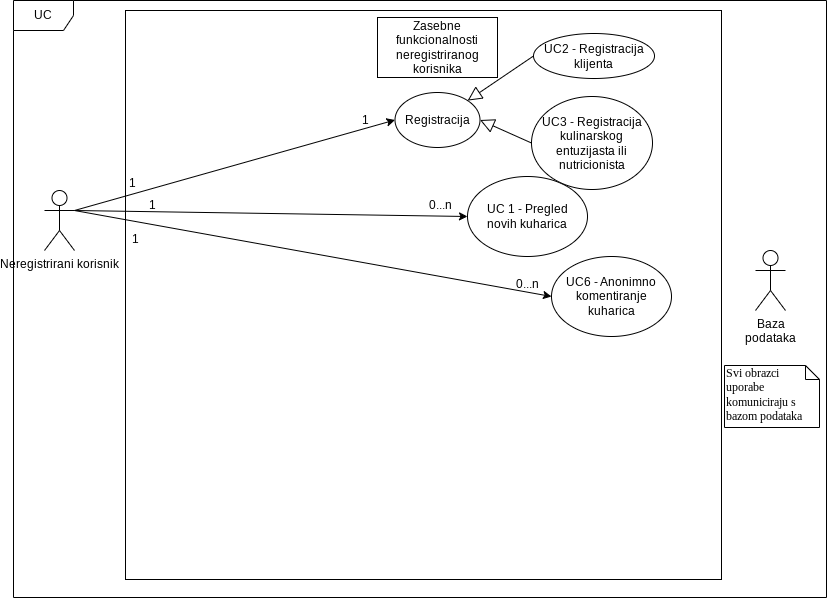
\includegraphics[scale=0.5]{dijagrami/dijagram-obrazaca-uporabe-neregistriranog-korisnika.png}
						\caption{Dijagram obrasca uporabe za neregistriranog korisnika}
						\label{fig:uc-neregistrirani}
					\end{figure}
					\begin{figure}[H]
						\centering
						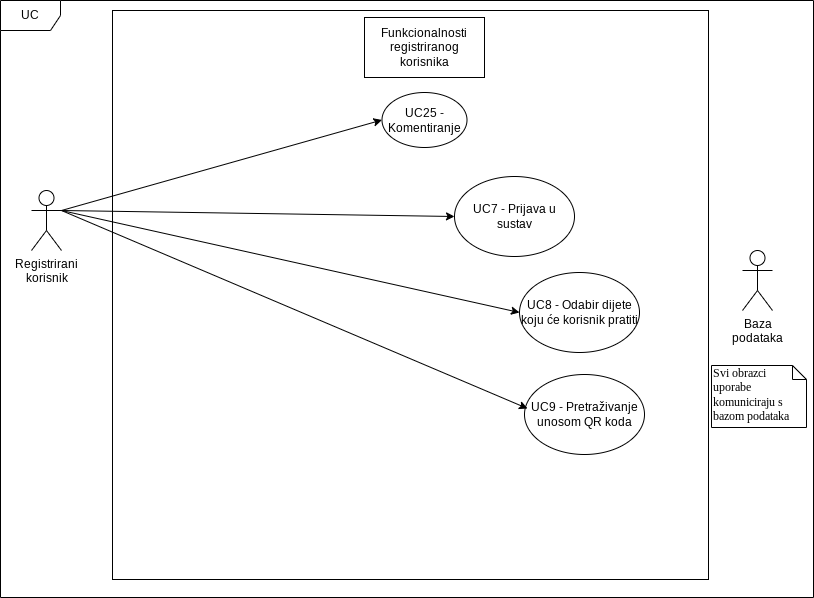
\includegraphics[scale=0.5]{dijagrami/dijagram-obrazaca-uporabe-registriranog-korisnika.png}
						\caption{Dijagram obrasca uporabe za registriranog korisnika}
						\label{fig:uc-registrirani}
					\end{figure} 
					\begin{figure}[H]
						\centering
						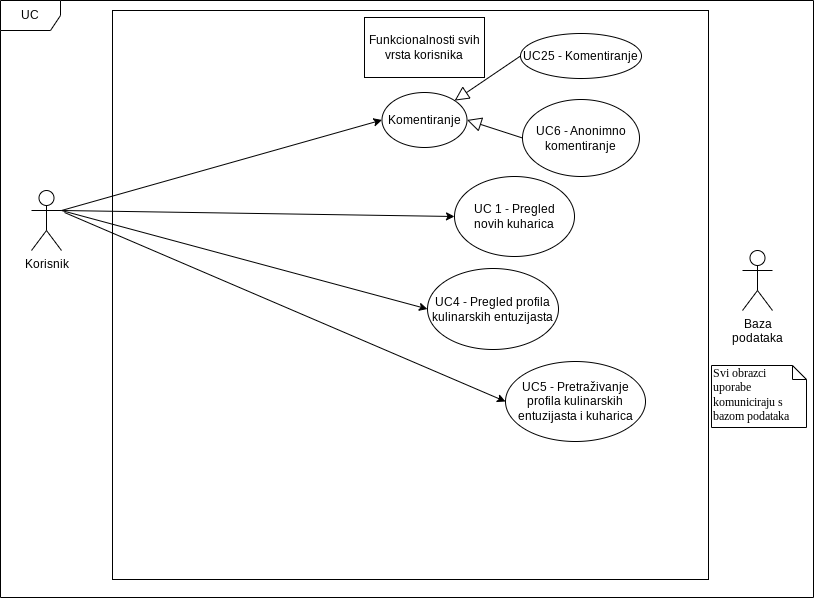
\includegraphics[scale=0.5]{dijagrami/dijagram-obrazaca-uporabe-za-sve-korisnike.png}
						\caption{Dijagram obrasca uporabe zajedničkog za sve korisnike}
						\label{fig:uc-svi-korisnici}
					\end{figure}
					\begin{figure}[H]
						\centering
						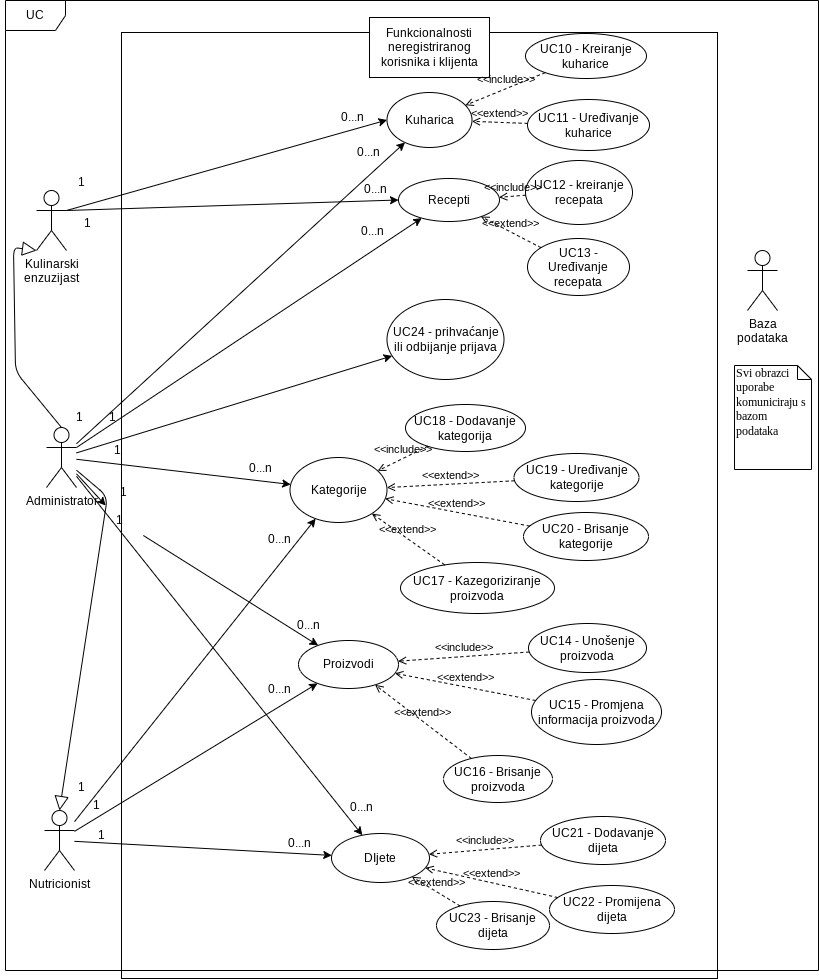
\includegraphics[scale=0.5]{dijagrami/dijagram-obrazaca-uporabe-kulinarskog-entuzijasta-i-nutricionista.png}
						\caption{Dijagram obrasca uporabe za kulinarskog entuzijasta i nutricionista}
						\label{fig:uc-kulinarski-i-nutricionist}
					\end{figure}
%					\textit{Prikazati odnos aktora i obrazaca uporabe odgovarajućim UML dijagramom. Nije nužno nacrtati sve na jednom dijagramu. Modelirati po razinama apstrakcije i skupovima srodnih funkcionalnosti.}

				\eject		
				
			\subsection{Sekvencijski dijagrami}
					\begin{figure}[H]
						\centering
						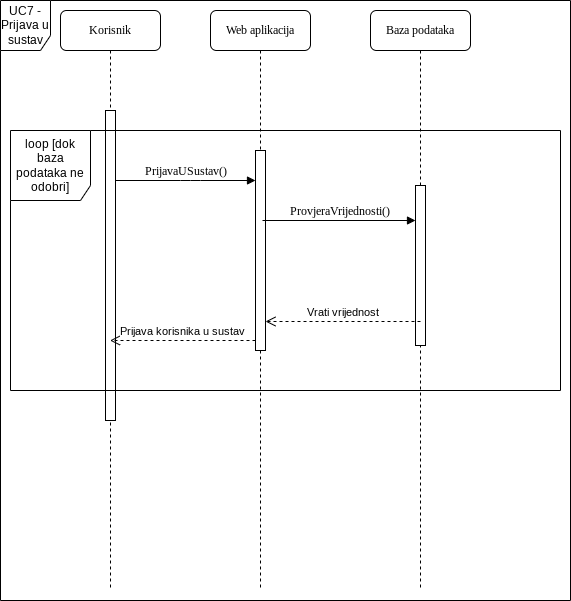
\includegraphics[scale=0.5]{dijagrami/sekvencijski-dijagram-prijave-u-sustav.png}
						\caption{Sekvencijski dijagram prijave u sustav}
						\label{fig:sekv-prijava}
					\end{figure}
					\subsubsection{Opis dijagrama}
						Korisnik u sučelju za prijavu u sustav upisuje potrebne podatke. Web aplikacija unesene podatke šalje bazi podataka. Baza podataka, nakon provjere postoji li par vrijednosti username - password među spremljenim vrijednostima, šalje poruku potvrde ili negacije postojanja para vrijednosti među podatcima. Web aplikacija nakon primanja potvrde dopušta prijavu, a nakon primanja dobijanja informira korisnika o neispravnosti podataka i ostaje u sučelju za prijavu gdje korisnik može ponoviti postupaks. 
					
					\begin{figure}[H]
						\centering
						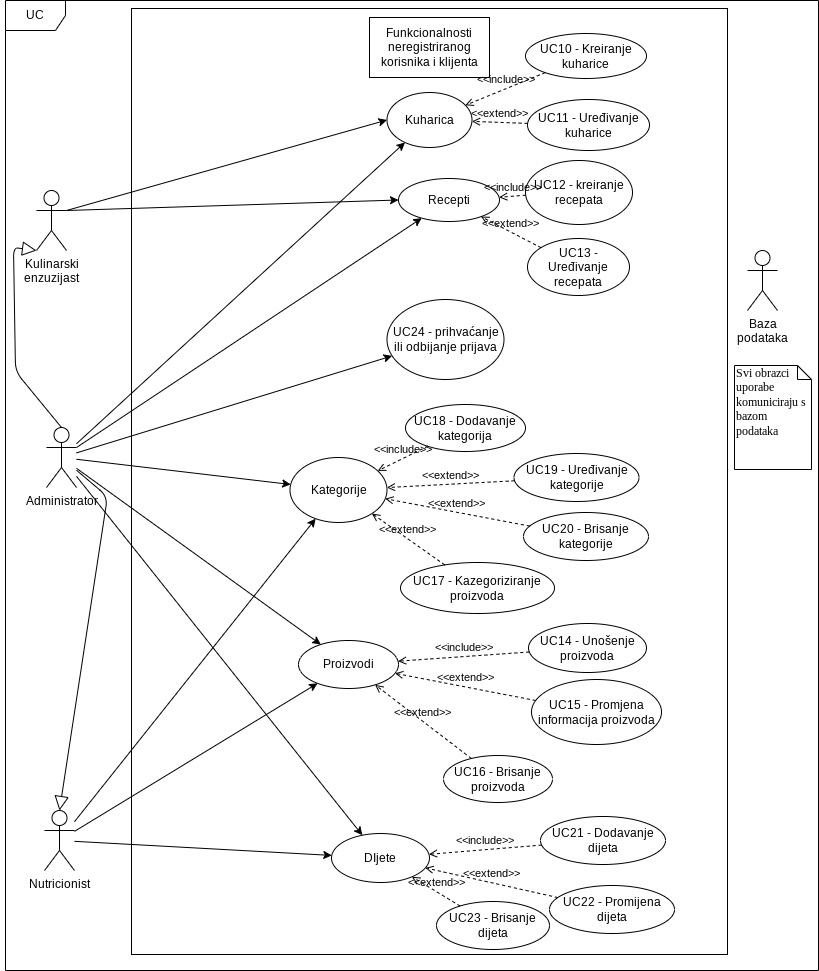
\includegraphics[scale=0.5]{dijagrami/sekvencijski-dijagram-registracije-nutricionista-i-kulinarskih-entuzijasta.png}
						\caption{Sekvencijski dijagram-registracije nutricionista i kulinarskih entuzijasta}
						\label{fig:sekv-registracija}
					\end{figure}
					\subsubsection{Opis dijagrama}
						Korisnik u sučelju za registraciju nutricionista ili kulinarskog entuzijasta unosi potrebne podatke. Nakon predaje registracije korisnik nastavlja koristiti web aplikaciju sa statusom klijenta. Web aplikacija podatke o registraciji šalje bazi podataka koja ih sprema. Nakon prijave administratora u sustav, baza podataka šalje podatke registracije web aplikaciji koja ih potom prikazuje administratoru. Administrator pregledava priložene informacije i odobrava ili odbija registraciju korisnika. Web aplikacija podatke o odluci  šalje bazi podataka koja bazirano na njima ima priliku promijeniti status korisnika. Nakon primanja podataka, baza podataka šalje informacije web aplikaciji koja prilaže informacije korisniku o uspješnoj registraciji ili o neuspješnoj registraciji i pruža korisniku priliku da izmijeni unesene podatke. 





%				\textbf{\textit{dio 1. revizije}}\\
%				
%				\textit{Nacrtati sekvencijske dijagrame koji modeliraju najvažnije dijelove sustava (max. 4 dijagrama). Ukoliko postoji nedoumica oko odabira, razjasniti s asistentom. Uz svaki dijagram napisati detaljni opis dijagrama.}
				\eject
	
		\section{Ostali zahtjevi}
			\begin{packed_item}
				\item Potrebno je omogućiti rad više korisnika u isto vrijeme.
				\item Sustav mora biti implementiran web aplikacijom
				\item Osjetljivi podatci poput lozinki moraju biti pohranjeni na adekvatan način, to jest kriptirani
				\item Korisničko sučelje mora biti otporno na pogreške tijekom korištenja
				\item Sustav mora biti javno dostupan putem web domene 
				\item Promet koji razmjenjuju klijent i poslužitelj mora biti zaštićen protokolom HTTPS
				\item Aplikacija mora biti razvijena koristeći objektno-orijentiranu paradigmu
			\end{packed_item}
%			\textbf{\textit{dio 1. revizije}}\\
%		 
%			 \textit{Nefunkcionalni zahtjevi i zahtjevi domene primjene dopunjuju funkcionalne zahtjeve. Oni opisuju \textbf{kako se sustav treba ponašati} i koja \textbf{ograničenja} treba poštivati (performanse, korisničko iskustvo, pouzdanost, standardi kvalitete, sigurnost...). Primjeri takvih zahtjeva u Vašem projektu mogu biti: podržani jezici korisničkog sučelja, vrijeme odziva, najveći mogući podržani broj korisnika, podržane web/mobilne platforme, razina zaštite (protokoli komunikacije, kriptiranje...)... Svaki takav zahtjev potrebno je navesti u jednoj ili dvije rečenice.}
			 
			 
			 
	